\documentclass[doc,floatsintext]{apa6}
\usepackage[american]{babel}
\usepackage{csquotes}
\usepackage{apacite}
\usepackage[T1]{fontenc}
\usepackage{lmodern}
\usepackage[utf8]{inputenc}
\usepackage{amssymb}
\usepackage{amsfonts}
\usepackage{amsmath}
\usepackage{graphicx}
\usepackage{float}
\usepackage{caption}
\usepackage{subcaption}
\usepackage{enumitem}
\usepackage[section]{placeins}
\usepackage[textsize=tiny]{todonotes}
\bibliographystyle{apacite}
\setlength{\marginparwidth}{2cm}

% ---------- watermark -----------
\usepackage[firstpage]{draftwatermark}
\SetWatermarkAngle{0}
\SetWatermarkFontSize{0.25cm}
\SetWatermarkVerCenter{0.75cm}
\SetWatermarkLightness{0.5}
\SetWatermarkHorCenter{14cm}
\SetWatermarkText{\shortstack[l]{
Navarro, D. J. (2004). A note on the applied use of MDL approximations \\
Neural Computation, 16, 1763-1768. http://dx.doi.org/10.1162/0899766041336378
}}
\SetWatermarkScale{1}
% -------------------------------

\title{A note on the applied use of MDL approximations}
\author{\normalsize Danielle J. Navarro}
\affiliation{Department of Psychology \\ Ohio State University}
\date{}
\shorttitle{}

\abstract{An applied problem is discussed in which two nested psychological models of retention are compared using Minimum Description Length (MDL). The standard Fisher information approximation (FIA) to the Normalized Maximum Likelihood (NML) is calculated for these two models, with the result that the full model is assigned a smaller complexity, even for moderately large samples. A geometric interpretation for this behavior is considered, along with its practical implications.}

\begin{document}
\maketitle

\vspace*{10pt}
The Minimum Description Length (MDL) principle (Rissanen 1978; see also Gr\"{u}nwald 1998) has attracted interest in applied fields, because it allows comparisons between non-nested and misspecified models without requiring restrictive assumptions. Of particular interest is the Normalized Maximum Likelihood (NML) criterion,

\begin{displaymath}
\mbox{NML} = \frac{p(X|\theta^\ast(X))}{\int p(Y|\theta^\ast(Y)) \ dY}
\end{displaymath}

\noindent
where $\theta^\ast(X)$ denotes the maximum likelihood estimate (MLE) for the data $X$. While the NML has many desirable properties (Rissanen 2001), a practical difficulty is that the normalization term is difficult to evaluate. Consequently, an approach based on Fisher information (FIA) is often used in its place (e.g. Rissanen 1996). This criterion is given by,

\begin{displaymath}
\mbox{FIA} = -\ln p(X|\theta^\ast(X)) + \frac{k}{2} \ln \left(\frac{N}{2\pi}\right) + \ln \int \sqrt{|I(\theta)|} \,\, d\theta + o(1)
\end{displaymath}

\noindent
where $k$ denotes the number of free parameters, $N$ denotes the sample size, and $I(\theta)$ denotes the expected Fisher information matrix of sample size one. The second and third terms are often referred to as a complexity penalty. Under regularity conditions\footnote{ The regularity conditions, most importantly the asymptotic normality of the MLE, are satisfied for models that constitute compact (i.e. closed and bounded) subsets of an exponential family, such as those discussed here.}  (Rissanen 1996, p.\ 41-42), it can be shown that the FIA asymptotically converges to $-\ln(\mbox{NML})$. %\setlength{\baselineskip}{24pt}

%\footnote{The required conditions are discussed by Takeuchi (in press). For the purposes of this paper, it suffices to note that the regularity conditions are satisfied for models (such as those discussed subsequently) that constitute compact (i.e. closed and bounded) subsets of an exponential family.}

The practical advantage to the FIA is that it only requires integration over the parameter space, and that the Fisher information matrix is sometimes easier to find than the maximum likelihood. However, while the optimality of the NML criterion holds for all $N$, the FIA is only guaranteed asymptotically, which can be problematic in some applications. This note presents one such case. Since applied researchers are often forced by necessity to use asymptotic measures such as the FIA, it is useful to take note of circumstances under which they are inappropriate, and give consideration to the reasons.

\subsection*{The Applied Problem}

The applied problem originates in the study of human forgetting (``retention''; see Navarro, Pitt \& Myung, in press). In a typical retention experiment, participants are presented with a list of words, and asked to recall them later. Measurements at different times after stimulus presentation produce a ``retention curve'': The probability of accurate recall is initially high, but tends towards zero over time. A retention model takes the form $p(C|t) = f(t,\theta)$ where $p(C|t)$ denotes the probability of correct recall at time $t$, and $f(t,\theta)$ is the hypothesized form of the retention curve, parametrized by $\theta$. Obviously, $f(t,\theta)$ must lie on $[0, 1]$ for all $t$. Additionally, $t$ is normalized to lie between 0 and 1.

The classic retention model is the exponential (EX) model, $f(t, \theta)=a\exp(-bt)$, where $\theta = (a, b)$ such that $a \in [0,1]$ denotes the initial retention probability, and $b$ gives the decay rate. While definitive bounds on $b$ are not easy to specify, experience with a large database suggests that $[0,100]$ is reasonable (see Rubin \& Wenzel 1996 or Navarro et al., in press). A second retention model is provided by Wickelgren's (1972) ``strength-resistance'' (SR) theory, which hypothesizes that $f(t, \theta)=a\exp(-bt^w)$ where $\theta = (a, b, w)$. Importantly, $w$ is constrained to lie on $[0,1]$, since $w<0$ results in an increasing retention function, and $w>1$ results in a faster-than-exponential decay, neither of which is consistent with the theory. Note that the EX model is a special case of the SR model, and by inspection, the NML denominator term is always smaller for the EX model than for the SR model, irrespective of sample size.

\subsection*{Fisher Information Matrices}

In any retention experiment, continuous measurements are impractical, so retention is measured at some number $m$ of fixed time intervals $t_1,\ldots, t_m$. Thus the observed data may be treated as $N$ observations from an $m$-variate binomial distribution, where the $i$-th Bernoulli probability is described by $f(t_i, \theta)$. A standard result (e.g., Schervish 1995, p110-115; Su, Myung \& Pitt, in press) allows the $uv$-th element of the Fisher information matrix of sample size one for these models to be written

\begin{displaymath}
I_{uv}(\theta)= \sum_{i=1}^m \frac{1}{f(t_i, \theta)(1-f(t_i, \theta))} \frac{\partial f(t_i, \theta)}{\partial \theta_u} \frac{\partial f(t_i, \theta)}{\partial \theta_v}.
\end{displaymath}

\noindent
The partial derivatives of $f(t_i, \theta)$ are simple. For the EX model, $\partial f(t_i, \theta) / \partial a = \exp(-bt_i)$ and $\partial f(t_i, \theta) / \partial b = -at_i \exp(-bt_i)$. For the SR model, the partial derivatives are $\partial f(t_i, \theta) / \partial a = \exp(-bt_i^w)$, $\partial f(t_i, \theta) / \partial b = -at_i^w \exp(-bt_i^w)$, and $\partial f(t_i, \theta) / \partial w = -abt_i^w \ln(t_i) \exp(-bt_i^w)$. Substitution into the Fisher information formula yields

%\setlength{\baselineskip}{24pt}
\begin{displaymath}
I(a,b) = \left[ \begin{array}{cc} (1/a) \sum_{i=1}^m y(i) & -\sum_{i=1}^m t_i y(i)  \\ -\sum_{i=1}^m t_i y(i) & a \sum_{i=1}^m t_i^2 y(i) \end{array} \right]
\end{displaymath}
%\setlength{\baselineskip}{24pt}

\noindent
for the EX model, where $y(i)=1\left/ (\exp(bt_i) - a)\right.$. For the SR model,
%\setlength{\baselineskip}{24pt}

\footnotesize
\begin{displaymath}
I(a,b,w) = \left[ \begin{array}{ccc} (1/a) \sum_{i=1}^{m} z(i) & -\sum_{i=1}^{m} t_i^w z(i) & -b \sum_{i=1}^{m} t_i^w (\ln t_i) z(i) \\ -\sum_{i=1}^{m} t_i^w z(i) & a \sum_{i=1}^{m} t_i^{2w} z(i) & ab \sum_{i=1}^{m} t_i^{2w} (\ln t_i) z(i) \\ -b \sum_{i=1}^{m} t_i^w (\ln t_i) z(i) & ab \sum_{i=1}^{m} t_i^{2w} (\ln t_i) z(i) &  ab^2 \sum_{i=1}^{m} t_i^{2w} (\ln t_i)^2 z(i)\end{array} \right]
\end{displaymath}
\normalsize

\noindent
where $z(i)=1\left/ (\exp(bt_i^w) - a)\right.$.

%\setlength{\baselineskip}{24pt}
\subsection*{Small Sample Behavior}

The experimental design was assumed to consist of 8 evenly spaced $t_i$ values, though the results are consistent across a range of designs. Without a closed form for the integral in the FIA, numerical estimates were obtained using Monte Carlo methods (e.g. Robert \& Casella 1999). Given the low dimensionality of the integrals and the unnecessarily extensive sampling ($10^8$ samples were taken), even simple Monte Carlo methods provide adequate results. The integral term $\int \sqrt{|I(\theta)|} d\theta$ for the EX model is approximately 8.0817, whereas for the SR model the value is approximately 0.4426. Substituting this into the FIA expression indicates that the SR model has a higher estimated complexity only when $N\geq 2096$, as shown in Figure~\ref{fia}. This presents a substantial difficulty for the applied problem, since not one of the 77 data sets considered by Navarro et al.\ (in press) had a sample size this large. Therefore, every data set that could possibly be observed would be better fit by SR, yet the nested EX model would be penalized more severely for excess complexity.

\begin{figure}\begin{center}
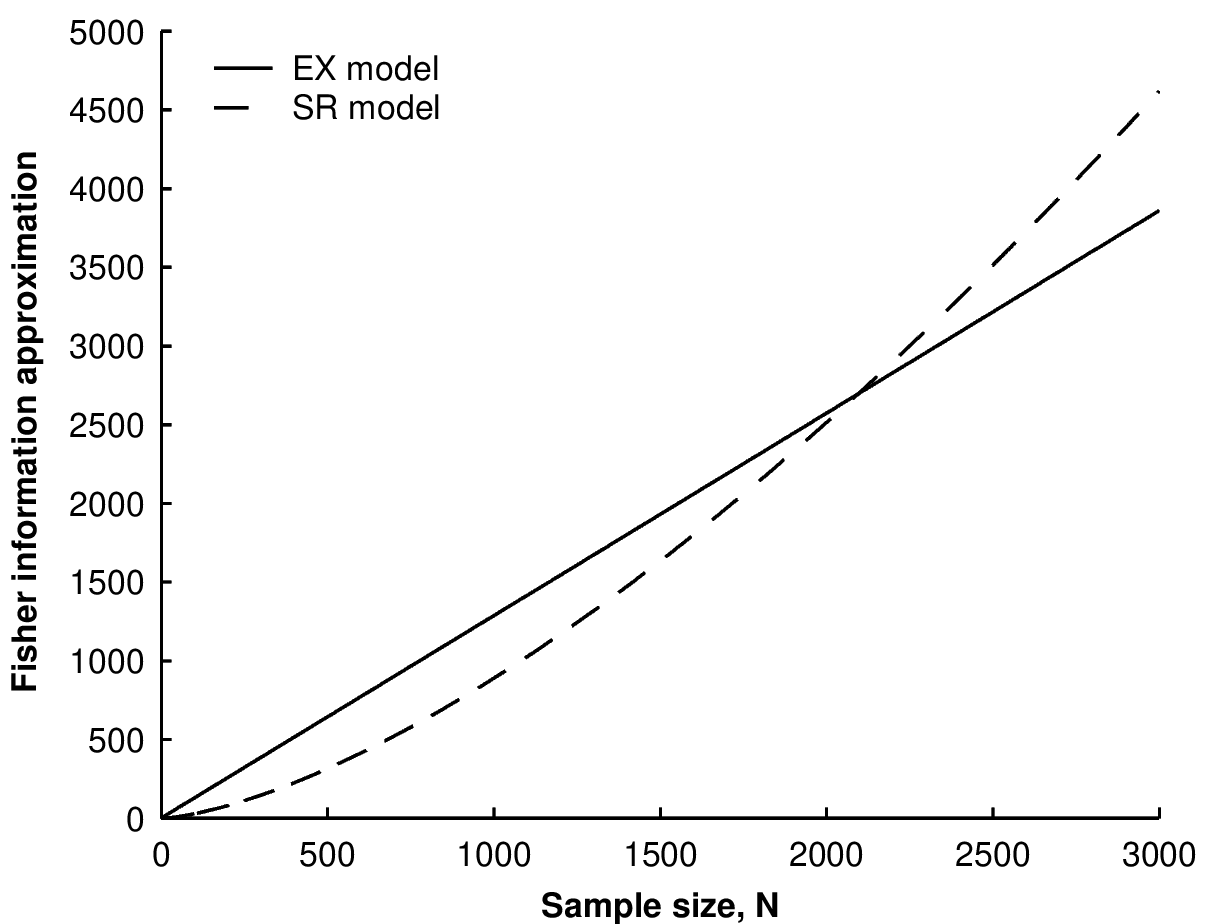
\includegraphics[width=8cm]{fia.png}
%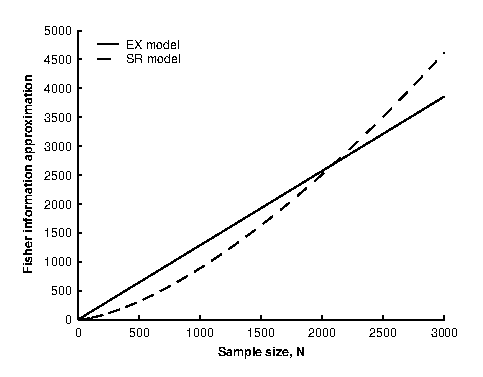
\epsfig{file=fia.eps,width=8cm}
\caption{The complexity assigned by the Fisher information approximation (FIA) for the EX and SR models (before taking logarithms).}
\label{fia}
\end{center}\end{figure}

It is worth considering the source of this problem. Following Myung, Balasubramanian and Pitt (2000) and Balasubramanian (1997), the complexity terms in the FIA can be viewed as approximations to (the logarithm of) the ratio of two Riemannian volumes. The first is the volume occupied by the model in the space of probability distributions (assuming the Fisher information metric), given by $V_f=\int \sqrt{|I(\theta)|} d\theta$. The second volume is that of a little ellipsoid around $\theta^\ast$, intended to quantify the size of a ``region of appreciable fit'', given by $V_c=\left(2\pi/N\right)^{k/2} \sqrt{|J(\theta^\ast)|/|I(\theta^\ast)|}$ where $J(\theta^\ast) = -1/N \left[ \sum_t\partial^2 \ln p(C|t) / \partial \theta_u \partial \theta_v \right]_{\theta = \theta^*}$ is the observed information. In general, the observed information $J(\theta^\ast)$ will differ from the expected information $I(\theta^\ast)$, but for the current purposes it suffices to note that there are data sets for which they are very similar, yielding $J(\theta^\ast) \approx I(\theta^\ast)$. As these are binomial models, an example of such a data set would be one in which $C_i \approx N f(t_i, \theta^*)$ for all $i$ since the data are almost identical to their expected values at the MLE parameters. Note that these are the data sets that are well fit by the model, and are thus precisely those of most interest to applied research. In such cases, $V_c \approx \left(2\pi/N\right)^{k/2}$.

When the observed information matrix closely approximates the expected information matrix, it is reasonable to view the complexity penalty for the FIA as approximately equivalent to $\ln \left(V_f \left/ V_c \right.\right)$. At $N=1$ we observe that, for the EX model, $V_c=2\pi < 8.0817 \approx V_f$. The little ellipsoid is smaller than the model, as it should be. However, by expanding the EX model into a third dimension, one obtains the SR model, for which $V_c=(2\pi)^{3/2} > 0.4426 \approx V_f$. The volume of the three dimensional ellipsoid is now \emph{larger} than the volume of the entire model. Taken together, these observations suggest that the extension of the model along the new dimension induced by the addition of the $w$ parameter is so tiny that the ``small'' ellipsoid now protrudes extensively, like a marble embedded in a sheet of paper. Most of the ``region of good fit'' no longer lies within the region occupied by the model. In short, until $N$ gets very large, $\theta^*$ does not seem to lie sufficiently within the model manifold to support the Gaussian approximations that underlie the FIA.

As an aside, it does not appear that the problem can be entirely solved by incorporating the $\sqrt{|J(\theta^\ast)|/|I(\theta^\ast)|}$ term. After all, by judicious choice of $t$ and $C$, data sets could be chosen for which the observed information is precisely equal to the expected information even at small samples. For instance, if $t=(.25, .5, .75, 1)$ and $N=16$, then the data set $C=(8, 4, 2, 1)$ yields MLE parameters $a^*=1$ and $b^*=\ln 16$ for both models, and $w^*=1$ for SR. In both cases, $f(t_i, \theta^*)=C_i/N$ for all $i$: The data take on their expected values at the MLE. Accordingly, $V_c = \left(2\pi/N\right)^{k/2}$ for these data. Even so, $V_f \approx 0.07$ for the SR model, while $V_f \approx 3.39$ for the EX model, indicating that the little ellipsoid is not well-located for the SR model.

\subsection*{Discussion}

Asymptotic approximations are useful in practice only insofar as they can be relied on to give the right answers. Clearly, if $V_c < V_f$ is not satisfied, the standard FIA expression is not necessarily reliable. In psychology, for instance, it is rare to find studies with $N>2000$, yet $V_c$ can still remain smaller than $V_f$ even at this sample size. This ``well-locatedness'' requirement is mentioned by Balasubramanian (1997) as a condition of his asymptotic expansions, but is not generally thought of as a regularity condition because it holds asymptotically (i.e. $V_c$ tends to zero as $N$ tends to infinity). In finite samples, some care is needed. While observing $V_c < V_f$ does not guarantee that $\theta^*$ is well-located, observing that $V_c > V_f$ does imply that it is not. It may be possible to use this observation to formulate approximations that perform better in small samples, though this question is left to more theoretically-inclined researchers.

In any case, it is clear that the source of the current difficulty does not lie with the MDL principle itself: The NML criterion does not suffer from this problem at any $N$. It is only that the $o(1)$ term in the asymptotic criterion can be large enough to make the approximation impractical for smaller samples. While the point is somewhat obvious, it does imply the need to take care in the use of the criterion. To that end, it is worth ensuring that $V_c < V_f$ before using the approximation.


\subsection*{Acknowledgements}

This research was supported by NIH grant R01-MH57472, and by a grant from the Office of Research at OSU. The author would like to thank Peter Gr\"{u}nwald, Michael Lee, In Jae Myung, and Mark Pitt for helpful suggestions, and two anonymous reviewers for comments that substantially improved the manuscript.


\subsection*{References}


\begin{list}
{}{\setlength{\leftmargin}{10pt}\setlength{\itemindent}{-10pt}\setlength{\parsep}{0pt}}
\item Balasubramanian, V. (1997). Statistical inference, Occam's razor and statistical mechanics on the space of probability distributions. {\it Neural Computation, 9}, 349-368.
\item Gr\"{u}nwald, P. (1998). {\it The Minimum Description Length Principle and Reasoning under Uncertainty}. Ph.D. Thesis, ILLC Dissertation Series DS 1998-03, CWI, the Netherlands.
\item Myung, I. J., Balasubramanian, V., \& Pitt, M. A. (2000). Counting probability distributions: Differential geometry and model selection. {\it Proceedings of the National Academy of Sciences USA, 97}, 11170-11175.
\item Navarro, D. J., Pitt, M. A. \& Myung, I. J. (in press). Assessing the distinguishability of models and the informativeness of data. {\it Cognitive Psychology}.
\item Rissanen, J. (1978). Modeling by the shortest data description. {\it Automatica, 14}, 465-471.
\item Rissanen, J. (1996). Fisher information and stochastic complexity. {\it IEEE Transactions on Information Theory 42}, 40-47.
\item Rissanen, J. (2001). Strong optimality of the normalized ML models as universal codes and information in data. {\it IEEE Transactions on Information Theory 47}, 1712-1717.
\item Robert, C. P. \& Casella, G. (1999). {\it Monte Carlo Statistical Methods}. Springer: New York.
\item Rubin, D. C. \& Wenzel, A. (1996). One hundred years of forgetting: A quantitative description of retention. {\it Psychological Review, 103}, 734-760.
\item Schervish, M. J. (1995). {\it Theory of Statistics}. New York: Springer.
\item Su, Y., Myung, I. J. \& Pitt, M. A. (in press). Minimum description length and cognitive modeling. In P. Gr\"{u}nwald, I. J. Myung, I. J., \& M. A. Pitt (Eds.) {\it Advances in Minimum Description Length: Theory and Applications}. MIT Press.
\item Wickelgren, W. A. (1972). Trace resistance and decay of long-term memory. {\it Journal of Mathematical Psychology, 9}, 418-455.
\end{list}

\bibliography{djn}
\end{document}


